\documentclass[10pt, twocolumn]{article}

\usepackage[letterpaper, portrait, margin=1in]{geometry}
\usepackage{setspace}
\usepackage{graphicx}
\usepackage{float}
\usepackage{geometry}
\usepackage{amsmath}
\usepackage{amssymb}
\usepackage{caption}
\usepackage{multicol}
\usepackage{titlesec}
\usepackage{fontspec}
\usepackage{xpatch}
\usepackage{xcolor}

\usepackage{fancyhdr}
\pagestyle{fancy}
\fancyhf{}
\lhead{\color{gold} \bfseries $\blacktriangleright$ \leftmark}
\rhead{}
\lfoot{Emmanuel College Biology Department}
\rfoot{\thepage}

\definecolor{darkblue}{HTML}{004B87}
\definecolor{gold}{HTML}{F6BE00}
\definecolor{lightblue}{HTML}{00AEEF}

\usepackage[backend=biber,style=authoryear]{biblatex}

\usepackage{xparse}% for multiple optional parameters
\usepackage{ifoddpage}% get correct page number

\makeatletter
\let\oldfootcite=\footcite
\RenewDocumentCommand{\footcite}{O{}O{}m}{\checkoddpage
  \@ifundefined{citepage@#3}{}%
  {\ifnum\csname citepage@#3\endcsname<\oddpage@page\relax
      \global\expandafter\let\csname repeatcite@#3\endcsname=\relax
  \fi}%
  \@ifundefined{repeatcite@#3}%
  {\oldfootcite[#1][#2]{#3}%
    \expandafter\xdef\csname repeatcite@#3\endcsname{\thefootnote}%
    \expandafter\xdef\csname citepage@#3\endcsname{\arabic{page}}}%
  {\footnotemark[\csname repeatcite@#3\endcsname]}}
\makeatother

\renewcommand{\headrulewidth}{2pt}
\renewcommand{\headrule}{\hbox to\headwidth{\color{darkblue}\leaders\hrule height \headrulewidth\hfill}}
\renewcommand{\footrulewidth}{2pt}
\renewcommand{\footrule}{\hbox to\headwidth{\color{gold}\leaders\hrule height \headrulewidth\hfill}}


% Some general changes
\DeclareNameAlias{sortname}{last-first}
\renewcommand*{\bibinitdelim}{}
\renewbibmacro*{in:}{%
    \iffieldequalstr{entrytype}{inproceedings}{%
        \printtext{\bibstring{in}\addspace}%
    }{}%
}

% Changes for Book
\csletcs{abx@macro@publisher+location+date@orig}{abx@macro@publisher+location+date}
\renewbibmacro*{publisher+location+date}{%
    \printtext[parens]{\usebibmacro{publisher+location+date@orig}}
}
\DeclareFieldFormat[book]{title}{#1\printunit{\addspace}}

% Changes for inproceedings
\DeclareFieldFormat[inproceedings]{title}{#1\isdot}
\DeclareFieldFormat{booktitle}{#1\addcomma}
\xpatchbibmacro{byeditor+others}{%
    \usebibmacro{byeditor+othersstrg}%
    \setunit{\addspace}%
    \printnames[byeditor]{editor}%
    \clearname{editor}%
}{%
    \printnames[byeditor]{editor}%
    \clearname{editor}
    \addcomma\addspace
    \bibstring{editor}
    \setunit{\addspace}%
}{}{}

% Changes in Article
\DeclareFieldFormat[article]{title}{#1}
\DeclareFieldFormat[article]{journaltitle}{#1\isdot}
\DeclareFieldFormat[article]{volume}{\textit{#1}}
\DeclareFieldFormat[article]{pages}{#1}

\setmainfont{Source Sans 3}

\titleformat{\section}[hang]{\large\bfseries\color{lightblue}}{\thesection}{0.5 em}{}{}

\titleformat{\subsection}[hang]{\normalsize\bfseries\color{lightblue}}{\thesubsection}{0.5 em}{}{}

\titleformat{\subsubsection}[hang]{\normalsize\bfseries\color{gold}}{~}{0.5 em}{}{}


\newcommand{\gitemp}[2] {\samepage{\noindent\textbf{\color{darkblue} $ \blacktriangleright $ {#1}} \\ {#2}} \smallskip}

\newcommand{\gitemn}[2] {\samepage{\noindent\textbf{\color{gray} $ \blacktriangleleft $ {#1}} \\ {#2}} \smallskip} 

\addbibresource{references.bib}

\title{A Review of Inclusive Practices and Language to Advance Scientific Identity of Marginalized Undergraduate Biology Students}
\author{Mickey Barron; Dr. Janel Cabrera, PhD}
\date{Emmanuel College \\ ~ \\ 2021-12-06}

\begin{document}

\begingroup

    \onecolumn

    \maketitle

    \abstract{This paper had a goal to do a thing and it acheived that thing with relative success.}

    \tableofcontents

    \twocolumn


\endgroup

\section{Introduction}

    This review was developed in order to promote diversity, equity, and inclusion (DEI) within the undergraduate biology and/or science, technology, engineering, and mathematics (STEM) settings. Specifically, this review aims to provide literature and recommendations to advance marginalized students' scientific identity (Sci-ID). Moreover, this review proposes an extension of the definition of Sci-ID drawing from the principles of computational identity (CI).

    \subsection{Scientific identity}

        Scientific identity (Sci-ID) is broadly defined as an identity model of one's inner sense of their alignment with science: whether or not they are a ``science person''.\footcite{salehjee_models_2018} \cite{oseguera_examining_2019} found that Black students had significantly lower Sci-ID than their white counterparts and identified that Sci-ID is a strong predictor of persistance in science. Moreover, the study found that intervention targeted towards improving Black students' Sci-ID is successful in raising Sci-ID to levels comparable to their white counterparts.\footcite{oseguera_examining_2019}
        
        Sci-ID development, therefore, is important to understand. \cite{salehjee_models_2018} establishes a seven-domain conjugated model of Sci-ID development. Sci-ID is influenced by: (1) global forces, such as one's identity, (2) social agencies and agents, such as educational institutes, teachers, and parents, (3) transformational learning experiences, including accidental and planned events that shapes one's perception of science, (4) one's openness to new information, (5) personal preference that selects for favored learning experiences, (6) individual internal agency, or one's internal drive to develop their Sci-ID, and (7) their core identity, which can be stable or fluid. Sci-ID develops as information is directed by domains 1-3 through domains 4-6 that act as filters that select for information to ultimately act upon domain 7, the core Sci-ID.\footcite{salehjee_models_2018}

        Sci-ID's development is well defined, however, Sci-ID itself varies in definition across literature. Thus, this review proposes a three-part definition drawing upon an analog from computer science: computational identity (CI). \cite{brousseau_position_2019} defines CI as a key factor in students' persistance in the pursuit of computing comprising of three components: (1) the perception that computing is useful, (2) self-efficacy in computing, and (3) a sense of belonging in computing.\footcite{brousseau_position_2019} Using this definition, this paper proposes a generalization of CI to Sci-ID, defining Sci-ID by three analogous components: (1) the perception that science is useful, (2) self-efficacy in science, and (3) a sense of belonging in science.\footcite{brousseau_position_2019} This definition is summarized in figure \ref{fig:sci_id}.

        \begin{figure}[h]
            \rule{\columnwidth}{1pt}
            \begin{center}
            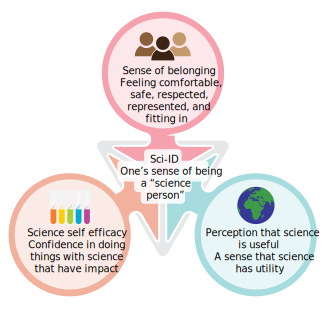
\includegraphics[width = \columnwidth]{figures/sci-id.pdf}
            \end{center}
            \caption{\textbf{Defining scientific identity (Sci-ID): a three-component system.} This diagram summarizes the definition of Sci-ID and its three components: (1) the perception that science is useful, (2) science self efficacy, and (3) a sense of belonging in science.}
            \label{fig:sci_id}
            \rule{\columnwidth}{1pt}
        \end{figure}

        \subsubsection{Perception that science is useful}

            An integral aspect of one's Sci-ID is one's perception that science is useful, in other words, they must have a sense that science is ``worth doing''. Moreover, one must feel that science is functional and applicable to their life. This is important as, per Eccles' expectancy-value theory\footcite{wigfield_expectancyvalue_2000}, the higher a student's subjective task value for science (their perception of the value and utility of learning and doing science), the more motivated they are to persist in science.\footcite{brousseau_position_2019} This perception that science is useful is critical to one's Sci-ID as it directly impacts their motivation and persistence in science.

        \subsubsection{Science self efficacy}

            Another important piece of one's Sci-ID is their self-efficacy in science. Science self-efficacy is one's own confidence in their ability to do science.\footcite{ballen_enhancing_2017} To elaborate, it is one's sense that not only can they do science, but in combination with their perception that science is useful, the things they can do with science have utility and impact.\footcite{brousseau_position_2019}  \cite{bandura_perceived_1993} found that one's self efficacy is a strong indicator of one's anxiety, motivation, and performance in a given domain; high self-efficacy conflates with strong performance and motivation with minimized anxiety whereas low self-efficacy is accompanied by high anxiety, a lack of motivation, and poor performance.\footcite{bandura_perceived_1993} Thus, it becomes apparent that science self efficacy is critical to one's Sci-ID; their confidence in science directly impacts their motivation to persist and their performance.

        \subsubsection{Sense of belonging in science}

            \begin{figure*}[t!]
                \begin{center}
                \includegraphics[height = 0.35 \paperheight]{figures/sense_of_belonging.pdf}
                \end{center}
                \caption{\textbf{Model of belonging differs for privileged and marginalized students and is dictated by involvement, relationships, and environment.} This diagram, sourced from \cite{vaccaro_development_2016}, summarizes key components of a sense of belonging and how those differ between privileged and marginalized students across environment, relationships, and involvement. Privileged students are represented in red and marginalized students are represented in blue.}
                \label{fig:sense_of_belonging}
                \rule{\textwidth}{1pt}
            \end{figure*}

            A sense of belonging is critical to a student's Sci-ID.  A student's sense of belonging consists of two major components: comfortability and fitting in; these components manifest across three domains: environment, relationships, and involvement. Students feel as though they belong when they feel comfort with others and in their surroundings and that they fit in with others and their surroundings on their campus.\footcite{vaccaro_development_2016}
            
            Developing a sense of belonging differs between marginalized and privileged students. It is important to understand how to support a sense of belonging for both types of students.\footcite{vaccaro_development_2016} Figure \ref{fig:sense_of_belonging} summarizes the key elements of the development of the sense of belonging and how it differs between privileged and marginalized students across the three domains. \cite{vaccaro_development_2016} found key differences emerge when analyzing the sense of belonging for marginalized students. In addition to feeling comfortable and fitting in, marginalized students value safety and respect where they feel physically safe in their settings, welcomed, accepted, and that both themself and their culture are respected.\footcite{vaccaro_development_2016}

            Students' environment impacts their sense of belonging; this impact varies greatly between marginalized and privileged students. Privileged students feel a sense of belonging in environments in which they describe as friendly, fun, and comfortable; these students typically attribute a sense of belonging exclusively to positive descriptors regarding their environment. Marginalized students, however, typically feel a lack of belonging in their environment as a result of feeling like the ``only one'' due to a lack of campus diversity and a restriction of authenticity in their expression due to judgement from others and different treatment. Thus, marginalized students require support in their authentic expression and diverse representation to feel belonging in their environment.\footcite{vaccaro_development_2016}

            Relationships are critical to students' sense of belonging. Privileged students seek a sense of familiarity with others, having fun, and receiving support in tasks in order to feel a sense of belonging. Marginalized students, rather, require deep connection and the ability to be comfortably authentic in their relationships in order to have a sense of belonging. Moreover, marginalized students may actively reject relationships that do not embrace their authentic expression.\footcite{vaccaro_development_2016}

            Involvement, too, is crucial to students' sense of belonging. Again, privileged and marginalized students value different aspects of belonging in involvement. Privileged students value fun and enjoyable involvement and when their involvement has a perceivable impact. Marginalized students, on the other hand, require involvement that allows and encourages authentic expression. Further, marginalized students value involvement that fosters authentic conversations and connections. This sense of authenticity is critical for marginalized students; involvement that did not nurture this authenticity did not foster belonging for these students and often lead to these students discontinuing their involvement.\footcite{vaccaro_development_2016}

            A student's sense of belonging, too, is critical to their Sci-ID, and therefore their performance and persistance in science. It becomes apparent that this sense of belonging must be prioritized and nurtured along with the other aspects of marginalized students' Sci-ID

    \subsection{Nurturing scientific identities of marginalized students}
        
        Given the dependence of marginalized students' perserverance and performance in science on scientific identity (Sci-ID), it becomes increasingly apparent that educational institutions must nurture marginalized students' Sci-IDs. For the undergraduate sciences, this paper presents a glossary of diversity, equity, and inclusion (DEI)-oriented terms sourced from modern academic journals, domain-specific recommendations, and diversity-representative scientists to be used by undergraduate professors to nurture the Sci-ID of marginalized students and proposed studies to evaluate the efficacy of these recommendations and resources.

\section{The Glossary}
    
    The glossary was constructed from a review of literature. The glossary lists: \\

    \gitemp{inclusive terms}{ that are suggested for use by individuals that are not part of the community and/or identity being discussed which are denoted with a $\blacktriangleright$ and highlighting them in blue.}

    \gitemn{exclusive terms}{ that are not suggested for use by individuals that are not part of the community and/or identity being discussedthat do not identify with the identity in reference which are denoted with a $\blacktriangleleft$ and highlighting them in gray.}

    \noindent It should be noted that these classifications are based on their use by individuals who are not a part of the community and/or identity being discussed; Ultimately, individuals who identify with the identity and/or community being discussed should be listened to and their self-identified labels and chosen terminology should be used. Self-labelling and chosen terminology is, typically, a result of personal context, intersectionality, self-agency, and, in some cases, a form of resistance.\footcite{wagaman_self-definition_2016} It should be the right of individuals who identify with the identity and/or community to make these choices as it empowers them and centers their needs and autonomy in discussions regarding them. \footcite{botha_does_2021}
    
    Additionally, these classifications make no indication on the moral good or bad of the term they are describing, rather they indicate the general acceptability of using that term to describe the phenomenon.

    \subsection{General}

        \gitemp{equality}{the ideal that every individual receives the same amount of resources and opportunities.\footcite{frones_equity_2020}}

        \gitemp{equity}{the ideal that every individual is allocated a variable amount of resources and opportunities to (1) counterbalance any disadvantage not resulting from an individual's choice and (2) to reward or punish in proportion to an individual's contribution to an impact or outcome.\footcite{frones_equity_2020}}

        \gitemp{diversity}{the heterogeneity, in otherwords, the sense of individual uniqueness, of people as a result of each person's individual ideologies, identities and lived experiences.\footcite{kvam_defining_2018}}

        \gitemp{marginalization}{the act of a society deplatforming and pushing people away from economic, sociopolitical, and cultural participation on the basis of identity, lived experience, and/or ideology that ultimately results in a maintained power imbalance between the dominating and marginalized identities and leads to deterioration of marginalized persons. }

        \gitemp{accountability}{in the social justice context, an individual and/or group's sense of responsibility as a result of their identity both privileging them at the expense of the marginalization of a group and providing them agency to use their privilege to align with and support the marginalized group.\footcite{wooldridge_what_nodate}}

        \gitemp{personal accountability}{the actions taken by an individual to hold themselves accountable in advancing a collective approach towards tansforming higher oppressive systems. While this is important, personal accountability should not be the focus of accountability as it undermines accountability's emphasis of collective action.\footcite{wooldridge_what_nodate}}

        \gitemp{collective accountability}{the collective action taken by a privileged group to hold themselves accountable in dismantling large-scale oppressive systems.\footcite{wooldridge_what_nodate}}

        \gitemp{ally}{an advocate or supporter of margianalized groups who jabe a reasonable understanding of the inequities and discrimination margianalized groups face and recognize their part in perpetuating the status quo that ultimately opresses these groups. \footcite{nash_male_2021}}

        \gitemp{culture}{a learned and dynamic social and individual construct that is a descriptive part of one's identity that manifests at several different depths, affects one's social and biological behavior and interpretations and perceptions of others' behaviors, ranges in applicability from individual to global used to associate with a social group. Individuals who identify as a part of a culture may vary in their degree of association and which aspects of a culture they specifically associate with.\footcite{spencer-oatey_what_2012}}

        \gitemp{cultural appropriation}{the act of individuals who do not identify as part of a culture stealing expressions, artifacts, intellectual property, history, and ways of knowledge from said culture without permission. \footcite{howard_equity_2020} This can manifest itself in one of at least three forms: subject, content, and tangible object appropriation.\footcite{lalonde_does_2021}}

        \gitemp{cultural subject appropriation}{the representation of a culture by someone who is not part of that culture, such as a non-Indigenous person making a documentary on Indigenous peoples. \footcite{lalonde_does_2021}}

        \gitemp{cultural content appropriation}{the use of a culture's property as a part of a cultural outsider's work, such as a white Internet influencer's use of African American Vernacular English in their content. \footcite{lalonde_does_2021}}

        \gitemp{cultural tangible object appropriation}{the stealing of culturally-significant artifacts, human remains, and/or destruction of culturally-significant landmarks,\footcite{lalonde_does_2021} such as the desecration of the Black Hills, sacred to the Lakota Sioux, into Mount Rushmore.\footcite{cottrell_mind_2020}}

    \subsection{Race \& Ethnicity}    

        \gitemp{race}{generally understood as a completely social construct with no biological basis, it is the perceived patterns of physical differences used to differentiate groups of people.\footcite{clair_racism_2015}}

        \gitemp{ethnicity}{an identity predominantly identified by a perceived common ancestry, culture, and/or history.\footcite{clair_racism_2015}}

        \subsubsection{Race}

        \gitemp{racial discrimination}{the unequal treatment of different races.\footcite{clair_racism_2015}}

        \gitemp{racial inequality}{the unequal outcomes between different races as a result of racial discrimination.\footcite{clair_racism_2015}}

        \gitemp{racism}{distinctly different from racial discrimination and inequality, it is an ideology of racial domination in which presumed cultural and/or biological superiority is used to prescribe, justify, or incite inferior treatment of another racial group. \footcite{clair_racism_2015}}

        \gitemp{overt racism}{also known as explicit racism, an instance of racism where racist ideas are blatantly clear, for example, the use of racial slurs.\footcite{mosley_critical_nodate}}

        \gitemp{covert racism}{also known as implicit racism, it is an instance of racism where unconciously triggerred beliefs of inferiority, negative attitudes towards, or assumptions of another race causes acts of racial discrimination.\footcite{clair_racism_2015}}

        \gitemp{institutional racism}{while it can be overt, it is a typically covert form of racism that results from racist policies, systems, and general norms in an institution or system that discriminate against and/or exploit certain races.\footcite{clair_racism_2015}}
        
        \gitemp{racial trauma}{also referred to as race-based traumatic stress, it is the collective psychological, emotional, and physical chronic injury as a result of experiencing racism, including overt, covert, interpersonal, insitutional, and systemic racism.\footcite{mosley_critical_nodate}}    

        \gitemp{anti-Black}{an ideology comrpised of stereotypes, beliefs, assumtions, and connotations of Black people based on a perceived difference that simultaneously compels the discrimination and systemic marginalization\footcite{nighaoui_color_2017} of Black people while also disregarding Black institutions and policies.\footcite{noauthor_racial_nodate}}

        \subsubsection{Ethnicity}


    \subsection{Sex \& Gender}
        \subsubsection{Gender}

            \gitemp{gender identity}{One's identity of their inner sense alignment (or lack their of) on the gender spectrum.}

            \gitemp{gender expression}{One's way of representing their gender identity through any means.}

            \gitemp{cisgender}{An gender identity that describes one whose current gender identity aligns with their sex assigned at birth.}

            \gitemp{Transgender}{A gender identity that describes one whose current gender identity does not align with their sex assigned at birth.}


        \subsubsection{Anatomical sex}

            \gitemp{sex assigned at birth}{The sex assignment a person receives from a medical professional that typically correlates to their genital phenotype}

            \gitemp{assigned female at birth (AFAB)}{A person whose sex assignment at birth was female. Typically, this assignment is a result of the presence of a vagina, ovaries, and uterus.}
                
            \gitemp{assigned male at birth (AMAB)}{A person whose sex assignment at birth was male. Typically, this assignment is a result of the presence of a penis and testicles.}

            \gitemp{Intersex}{A person whose gential phenotype is indiscriminate between male and female sexes. Typically, this is any combination of the presence of a penis, vagina, testicles, ovaries, and/or uterus.}

        \subsubsection{Genetic sex}


    \subsection{Sexuality}

    \subsection{Ability \& Disability}

        \subsubsection{Deaf \& Hard of Hearing}


            \gitemp{Deaf}{Deaf, or ``big D'' Deaf, is a cultural identity of individuals with hearing loss that typically describes people that use sign language and are a part of Deaf culture.\footcite{leigh_deaf_2020}}

            \gitemp{deaf}{deaf, or ``little d'' deaf, is a medical diagnosis indicating their hearing loss makes it hard or impossible to understand spoken language through hearing alone.\footcite{leigh_deaf_2020}}

            \gitemn{hearing impared}{A term used to describe deaf and hard of hearing people that should be avoided as it focuses on what deaf and hard of hearing people cannot do rather than what they can do. \footcite{leigh_deaf_2020}}

            \gitemn{auditory handicap}{A term used to describe deaf and hard of hearing people that should be avoided as it only focuses on their hearing loss rather than the term Deaf which has more meaning than just ``cannot hear''. \footcite{leigh_deaf_2020}}

            \gitemn{deaf mute}{An offensive term used to describe deaf and hard of hearing people that should be avoided as it only focuses on their hearing loss rather than the term Deaf which has more meaning than just ``cannot hear''. \footcite{leigh_deaf_2020}}

            \gitemn{hearing handicapped}{A term used to describe deaf and hard of hearing people that should be avoided as it only focuses on their hearing loss rather than the term Deaf which has more meaning than just ``cannot hear''. \footcite{leigh_deaf_2020}}

            \gitemn{prelingually deaf}{A term used to describe deaf and hard of hearing people that should be avoided as it only focuses on their hearing loss rather than the term Deaf which has more meaning than just ``cannot hear''. \footcite{leigh_deaf_2020}}

            \gitemn{deaf and dumb}{An offensive term used to describe deaf and hard of hearing people that should be avoided as it only focuses on their hearing loss rather than the term Deaf which has more meaning than just ``cannot hear''. \footcite{leigh_deaf_2020}}

    \subsection{Socioeconomic Status}

\section{General recommendations}
    
    \subsection{War-related analogies}


\section{Disease Recommendations}

        \subsection{SARS-CoV-2 \& COVID-19}

\section{Genetics recommendations}

\section{Anatomy \& physiology recommendations}

\section{Noteworthy scientists of marginalized identities}

\section*{Acknowledgements}

The authors would like to sincerely thank Luz Padilla, Nadel Henville, and Liam Rice for referring sources to be used in this paper.

\printbibliography

\end{document}